\documentclass[border=8pt]{standalone}
\usepackage{fontspec}
\setsansfont{Arial}
\usepackage{pgfplots}
\usepgfplotslibrary{groupplots}
\pgfplotsset{compat=1.18,
  every axis/.append style={/pgf/number format/assume math mode=true,
    tick label style={font=\sffamily\small},
    nodes near coords style={font=\sffamily\scriptsize}}}
% Published-test AP and AR (%) by COCO object size for the frozen T41 pair.
% Source: docs/t41-results.md, Results table (PR #25).
\begin{document}
\sffamily\small
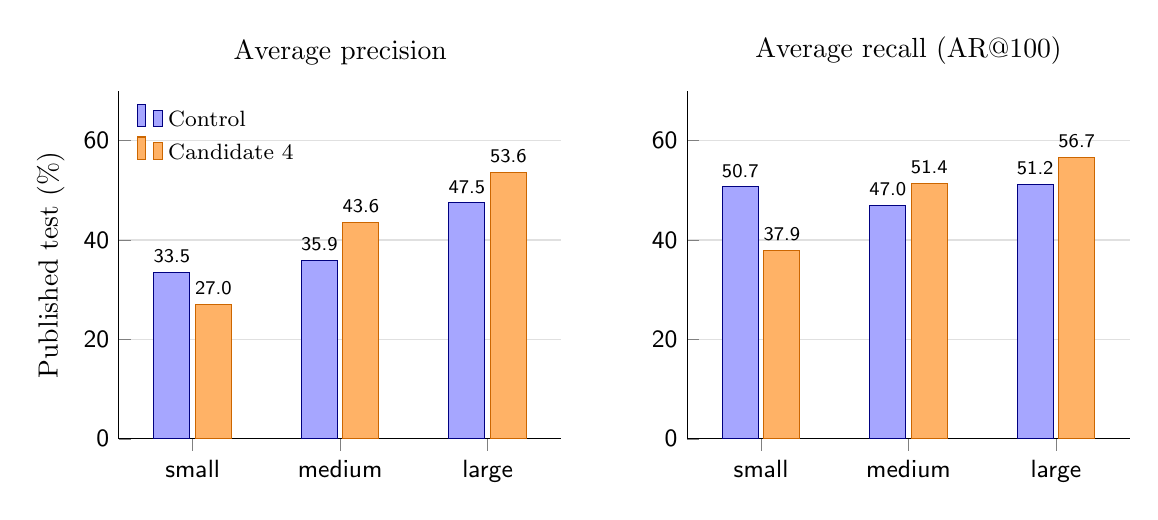
\begin{tikzpicture}
\begin{groupplot}[
  group style={group size=2 by 1,horizontal sep=1.6cm},
  width=7.2cm,height=6cm,
  ybar,/pgf/bar width=13pt,
  ymin=0,ymax=70,
  symbolic x coords={small,medium,large},
  xtick=data,
  enlarge x limits=0.25,
  nodes near coords,
  nodes near coords style={/pgf/number format/.cd,fixed,fixed zerofill,precision=1},
  ymajorgrids,grid style={black!12},
  axis lines*=left,
]
\nextgroupplot[title={Average precision},ylabel={Published test (\%)},
  legend style={font=\footnotesize,draw=none,fill=none,at={(0.02,0.98)},anchor=north west},
  legend cell align=left]
\addplot[fill=blue!35,draw=blue!50!black] coordinates
  {(small,33.4914) (medium,35.8683) (large,47.4741)};
\addplot[fill=orange!60,draw=orange!80!black] coordinates
  {(small,27.0458) (medium,43.5687) (large,53.5703)};
\legend{Control,Candidate 4}
\nextgroupplot[title={Average recall (AR@100)}]
\addplot[fill=blue!35,draw=blue!50!black] coordinates
  {(small,50.7018) (medium,46.9843) (large,51.2404)};
\addplot[fill=orange!60,draw=orange!80!black] coordinates
  {(small,37.8947) (medium,51.4295) (large,56.6816)};
\end{groupplot}
\end{tikzpicture}
\end{document}
